% Options for packages loaded elsewhere
\PassOptionsToPackage{unicode}{hyperref}
\PassOptionsToPackage{hyphens}{url}
\documentclass[
  10pt,
]{article}
\usepackage{xcolor}
\usepackage[margin=1in]{geometry}
\usepackage{authblk}
\usepackage{amsmath,amssymb}
\setcounter{secnumdepth}{-\maxdimen} % remove section numbering
\usepackage{iftex}
\ifPDFTeX
  \usepackage[T1]{fontenc}
  \usepackage[utf8]{inputenc}
  \usepackage{textcomp} % provide euro and other symbols
\else % if luatex or xetex
  \usepackage{unicode-math} % this also loads fontspec
  \defaultfontfeatures{Scale=MatchLowercase}
  \defaultfontfeatures[\rmfamily]{Ligatures=TeX,Scale=1}
\fi
\usepackage{lmodern}
\ifPDFTeX\else
  % xetex/luatex font selection
\fi
% Use upquote if available, for straight quotes in verbatim environments
\IfFileExists{upquote.sty}{\usepackage{upquote}}{}
\IfFileExists{microtype.sty}{% use microtype if available
  \usepackage[]{microtype}
  \UseMicrotypeSet[protrusion]{basicmath} % disable protrusion for tt fonts
}{}
\makeatletter
\@ifundefined{KOMAClassName}{% if non-KOMA class
  \IfFileExists{parskip.sty}{%
    \usepackage{parskip}
  }{% else
    \setlength{\parindent}{0pt}
    \setlength{\parskip}{6pt plus 2pt minus 1pt}}
}{% if KOMA class
  \KOMAoptions{parskip=half}}
\makeatother
\usepackage{color}
\usepackage{fancyvrb}
\newcommand{\VerbBar}{|}
\newcommand{\VERB}{\Verb[commandchars=\\\{\}]}
\DefineVerbatimEnvironment{Highlighting}{Verbatim}{commandchars=\\\{\}}
% Add ',fontsize=\small' for more characters per line
\newenvironment{Shaded}{}{}
\newcommand{\AlertTok}[1]{\textcolor[rgb]{1.00,0.00,0.00}{\textbf{#1}}}
\newcommand{\AnnotationTok}[1]{\textcolor[rgb]{0.38,0.63,0.69}{\textbf{\textit{#1}}}}
\newcommand{\AttributeTok}[1]{\textcolor[rgb]{0.49,0.56,0.16}{#1}}
\newcommand{\BaseNTok}[1]{\textcolor[rgb]{0.25,0.63,0.44}{#1}}
\newcommand{\BuiltInTok}[1]{\textcolor[rgb]{0.00,0.50,0.00}{#1}}
\newcommand{\CharTok}[1]{\textcolor[rgb]{0.25,0.44,0.63}{#1}}
\newcommand{\CommentTok}[1]{\textcolor[rgb]{0.38,0.63,0.69}{\textit{#1}}}
\newcommand{\CommentVarTok}[1]{\textcolor[rgb]{0.38,0.63,0.69}{\textbf{\textit{#1}}}}
\newcommand{\ConstantTok}[1]{\textcolor[rgb]{0.53,0.00,0.00}{#1}}
\newcommand{\ControlFlowTok}[1]{\textcolor[rgb]{0.00,0.44,0.13}{\textbf{#1}}}
\newcommand{\DataTypeTok}[1]{\textcolor[rgb]{0.56,0.13,0.00}{#1}}
\newcommand{\DecValTok}[1]{\textcolor[rgb]{0.25,0.63,0.44}{#1}}
\newcommand{\DocumentationTok}[1]{\textcolor[rgb]{0.73,0.13,0.13}{\textit{#1}}}
\newcommand{\ErrorTok}[1]{\textcolor[rgb]{1.00,0.00,0.00}{\textbf{#1}}}
\newcommand{\ExtensionTok}[1]{#1}
\newcommand{\FloatTok}[1]{\textcolor[rgb]{0.25,0.63,0.44}{#1}}
\newcommand{\FunctionTok}[1]{\textcolor[rgb]{0.02,0.16,0.49}{#1}}
\newcommand{\ImportTok}[1]{\textcolor[rgb]{0.00,0.50,0.00}{\textbf{#1}}}
\newcommand{\InformationTok}[1]{\textcolor[rgb]{0.38,0.63,0.69}{\textbf{\textit{#1}}}}
\newcommand{\KeywordTok}[1]{\textcolor[rgb]{0.00,0.44,0.13}{\textbf{#1}}}
\newcommand{\NormalTok}[1]{#1}
\newcommand{\OperatorTok}[1]{\textcolor[rgb]{0.40,0.40,0.40}{#1}}
\newcommand{\OtherTok}[1]{\textcolor[rgb]{0.00,0.44,0.13}{#1}}
\newcommand{\PreprocessorTok}[1]{\textcolor[rgb]{0.74,0.48,0.00}{#1}}
\newcommand{\RegionMarkerTok}[1]{#1}
\newcommand{\SpecialCharTok}[1]{\textcolor[rgb]{0.25,0.44,0.63}{#1}}
\newcommand{\SpecialStringTok}[1]{\textcolor[rgb]{0.73,0.40,0.53}{#1}}
\newcommand{\StringTok}[1]{\textcolor[rgb]{0.25,0.44,0.63}{#1}}
\newcommand{\VariableTok}[1]{\textcolor[rgb]{0.10,0.09,0.49}{#1}}
\newcommand{\VerbatimStringTok}[1]{\textcolor[rgb]{0.25,0.44,0.63}{#1}}
\newcommand{\WarningTok}[1]{\textcolor[rgb]{0.38,0.63,0.69}{\textbf{\textit{#1}}}}
\usepackage{longtable,booktabs,array}
\newcounter{none} % for unnumbered tables
\usepackage{calc} % for calculating minipage widths
% Correct order of tables after \paragraph or \subparagraph
\usepackage{etoolbox}
\makeatletter
\patchcmd\longtable{\par}{\if@noskipsec\mbox{}\fi\par}{}{}
\makeatother
% Allow footnotes in longtable head/foot
\IfFileExists{footnotehyper.sty}{\usepackage{footnotehyper}}{\usepackage{footnote}}
\makesavenoteenv{longtable}
\usepackage{graphicx}
\makeatletter
\newsavebox\pandoc@box
\newcommand*\pandocbounded[1]{% scales image to fit in text height/width
  \sbox\pandoc@box{#1}%
  \Gscale@div\@tempa{\textheight}{\dimexpr\ht\pandoc@box+\dp\pandoc@box\relax}%
  \Gscale@div\@tempb{\linewidth}{\wd\pandoc@box}%
  \ifdim\@tempb\p@<\@tempa\p@\let\@tempa\@tempb\fi% select the smaller of both
  \ifdim\@tempa\p@<\p@\scalebox{\@tempa}{\usebox\pandoc@box}%
  \else\usebox{\pandoc@box}%
  \fi%
}
% Set default figure placement to htbp
\def\fps@figure{htbp}
\makeatother
\setlength{\emergencystretch}{3em} % prevent overfull lines
\providecommand{\tightlist}{%
  \setlength{\itemsep}{0pt}\setlength{\parskip}{0pt}}
\usepackage{bookmark}
\IfFileExists{xurl.sty}{\usepackage{xurl}}{} % add URL line breaks if available
\urlstyle{same}
\hypersetup{
  pdftitle={PriorityKV: Structure-Aware KV Retention for Long Agent Traces},
  pdfauthor={Arush Sharma (IIT (ISM) Dhanbad); Anupam Rawart (IIT Bombay)},
  hidelinks,
  pdfcreator={LaTeX via pandoc}}

\title{PriorityKV: Structure-Aware KV Retention for Long Agent Traces}
\author[1]{Arush Sharma}
\author[2]{Anupam Rawart}
\affil[1]{Indian Institute of Technology (Indian School of Mines) Dhanbad}
\affil[2]{Indian Institute of Technology Bombay}
\date{}

\begin{document}
\maketitle

\begin{abstract}

Long language-model agent traces contain heterogeneous state: tool
schemas, system instructions, superseding constraints, identifiers,
ordinary dialogue, and filler. All of these tokens occupy the key-value
(KV) cache, but losing them has different behavioral consequences. We
study whether cache allocation should use this known trace structure. We
introduce PriorityBench-A, a locked 240-example benchmark covering
tool-schema conformance, instruction supersession, and multi-turn state
recall at 8k, 16k, and 32k context strata. On matched-budget eviction
stress slices, a role-blind sink-and-recent policy scores 0.000 while
structure-aware retention scores 1.000 at token granularity and 0.643 at
16-token page granularity. An adversarial buried-state variant lowers
the structure score to 0.429, identifying the boundary of the heuristic
rather than an oracle effect. We separately test mixed-precision storage
and falsify the hypothesis that soft INT4 quantization of 75\% of
positions creates a meaningful quality separation: on the locked 240
examples, FullKV, role-blind mixed, and structure-aware mixed score
0.888, 0.879, and 0.883, respectively. We therefore treat quantization
as a systems mechanism, not a quality result. Our Qwen3-8B prototype
stores BF16 and packed INT4 pages and uses FlashInfer-backed decode on
an H200. The structure-aware path uses 0.72x measured KV payload and
0.87x peak allocated CUDA memory relative to FullKV, while end-to-end
time to first token is 1.11--1.12x and time per output token is
1.20--1.21x. The gap between payload and peak is caused by an explicit
INT4-to-BF16 cold-attention scratch buffer. The result is a scoped
measurement study: agent-trace structure is useful under eviction, soft
INT4 is quality-neutral at the tested operating point, and packed bytes
do not automatically imply a latency or peak-memory win.
\end{abstract}

\section{1. Introduction}\label{1-introduction}

Autoregressive Transformer inference stores the keys and values of
previous tokens so that generation does not recompute the complete
prefix. The resulting KV cache grows with context length and batch size
and is a central memory-management concern in LLM serving {[}1, 2{]}.
Existing work reduces this cost through paging, eviction, token
selection, or quantization {[}2--9{]}. These methods generally
estimate token importance from position, attention, or activation
statistics.

Agent traces expose another signal before attention is evaluated: their
protocol structure. A serving layer often knows which spans are system
instructions, tool schemas, tool results, user constraints, or generated
dialogue. A role-blind cache policy can therefore satisfy a nominal
token budget while deleting state that is necessary for the
agent\textquotesingle s next action. Aggregate language-model metrics
may not expose failures such as a malformed tool call, compliance with
an obsolete instruction, or use of the wrong order identifier.

PriorityKV asks two questions:

\begin{enumerate}
\def\labelenumi{\arabic{enumi}.}
\tightlist
\item
  At a matched eviction budget, does preserving protocol structure
  improve agent-task reliability over role-blind position policies?
\item
  If low-precision KV storage is quality-neutral, can a working mixed
  BF16/INT4 cache still provide measurable systems value?
\end{enumerate}

These questions must remain separate. Eviction removes information;
quantization retains an approximation of it. Our initial expectation
that role-aware INT4 placement would create a quality gap was not
supported at the selected 75\% INT4 operating point. We keep that
negative result and evaluate the packed path in bytes and latency
instead.

This report makes four contributions:

\begin{enumerate}
\def\labelenumi{\arabic{enumi}.}
\tightlist
\item
  \textbf{PriorityBench-A:} a reproducible 240-example agent-reliability
  benchmark with deterministic scorers and a frozen manifest hash.
\item
  \textbf{Matched-budget eviction evidence:} structure-aware retention
  outperforms role-blind sink-and-recent and fixed-prefix controls on
  targeted stress slices, with an adversarial buried-state check that
  scopes the result.
\item
  \textbf{A falsified quality hypothesis:} uniform and structure-aware
  mixed INT4 policies remain close to FullKV on the locked 240-example
  evaluation.
\item
  \textbf{An auditable systems prototype:} packed BF16/INT4 pages,
  FlashInfer log-sum-exp state merging, phase-separated latency, and
  separate reporting of payload and peak memory on H200.
\end{enumerate}

The report does not claim paper-grade generalization across LongBench or
RULER, a quantization-driven accuracy advantage, or a fused INT4
attention speedup.

\pandocbounded{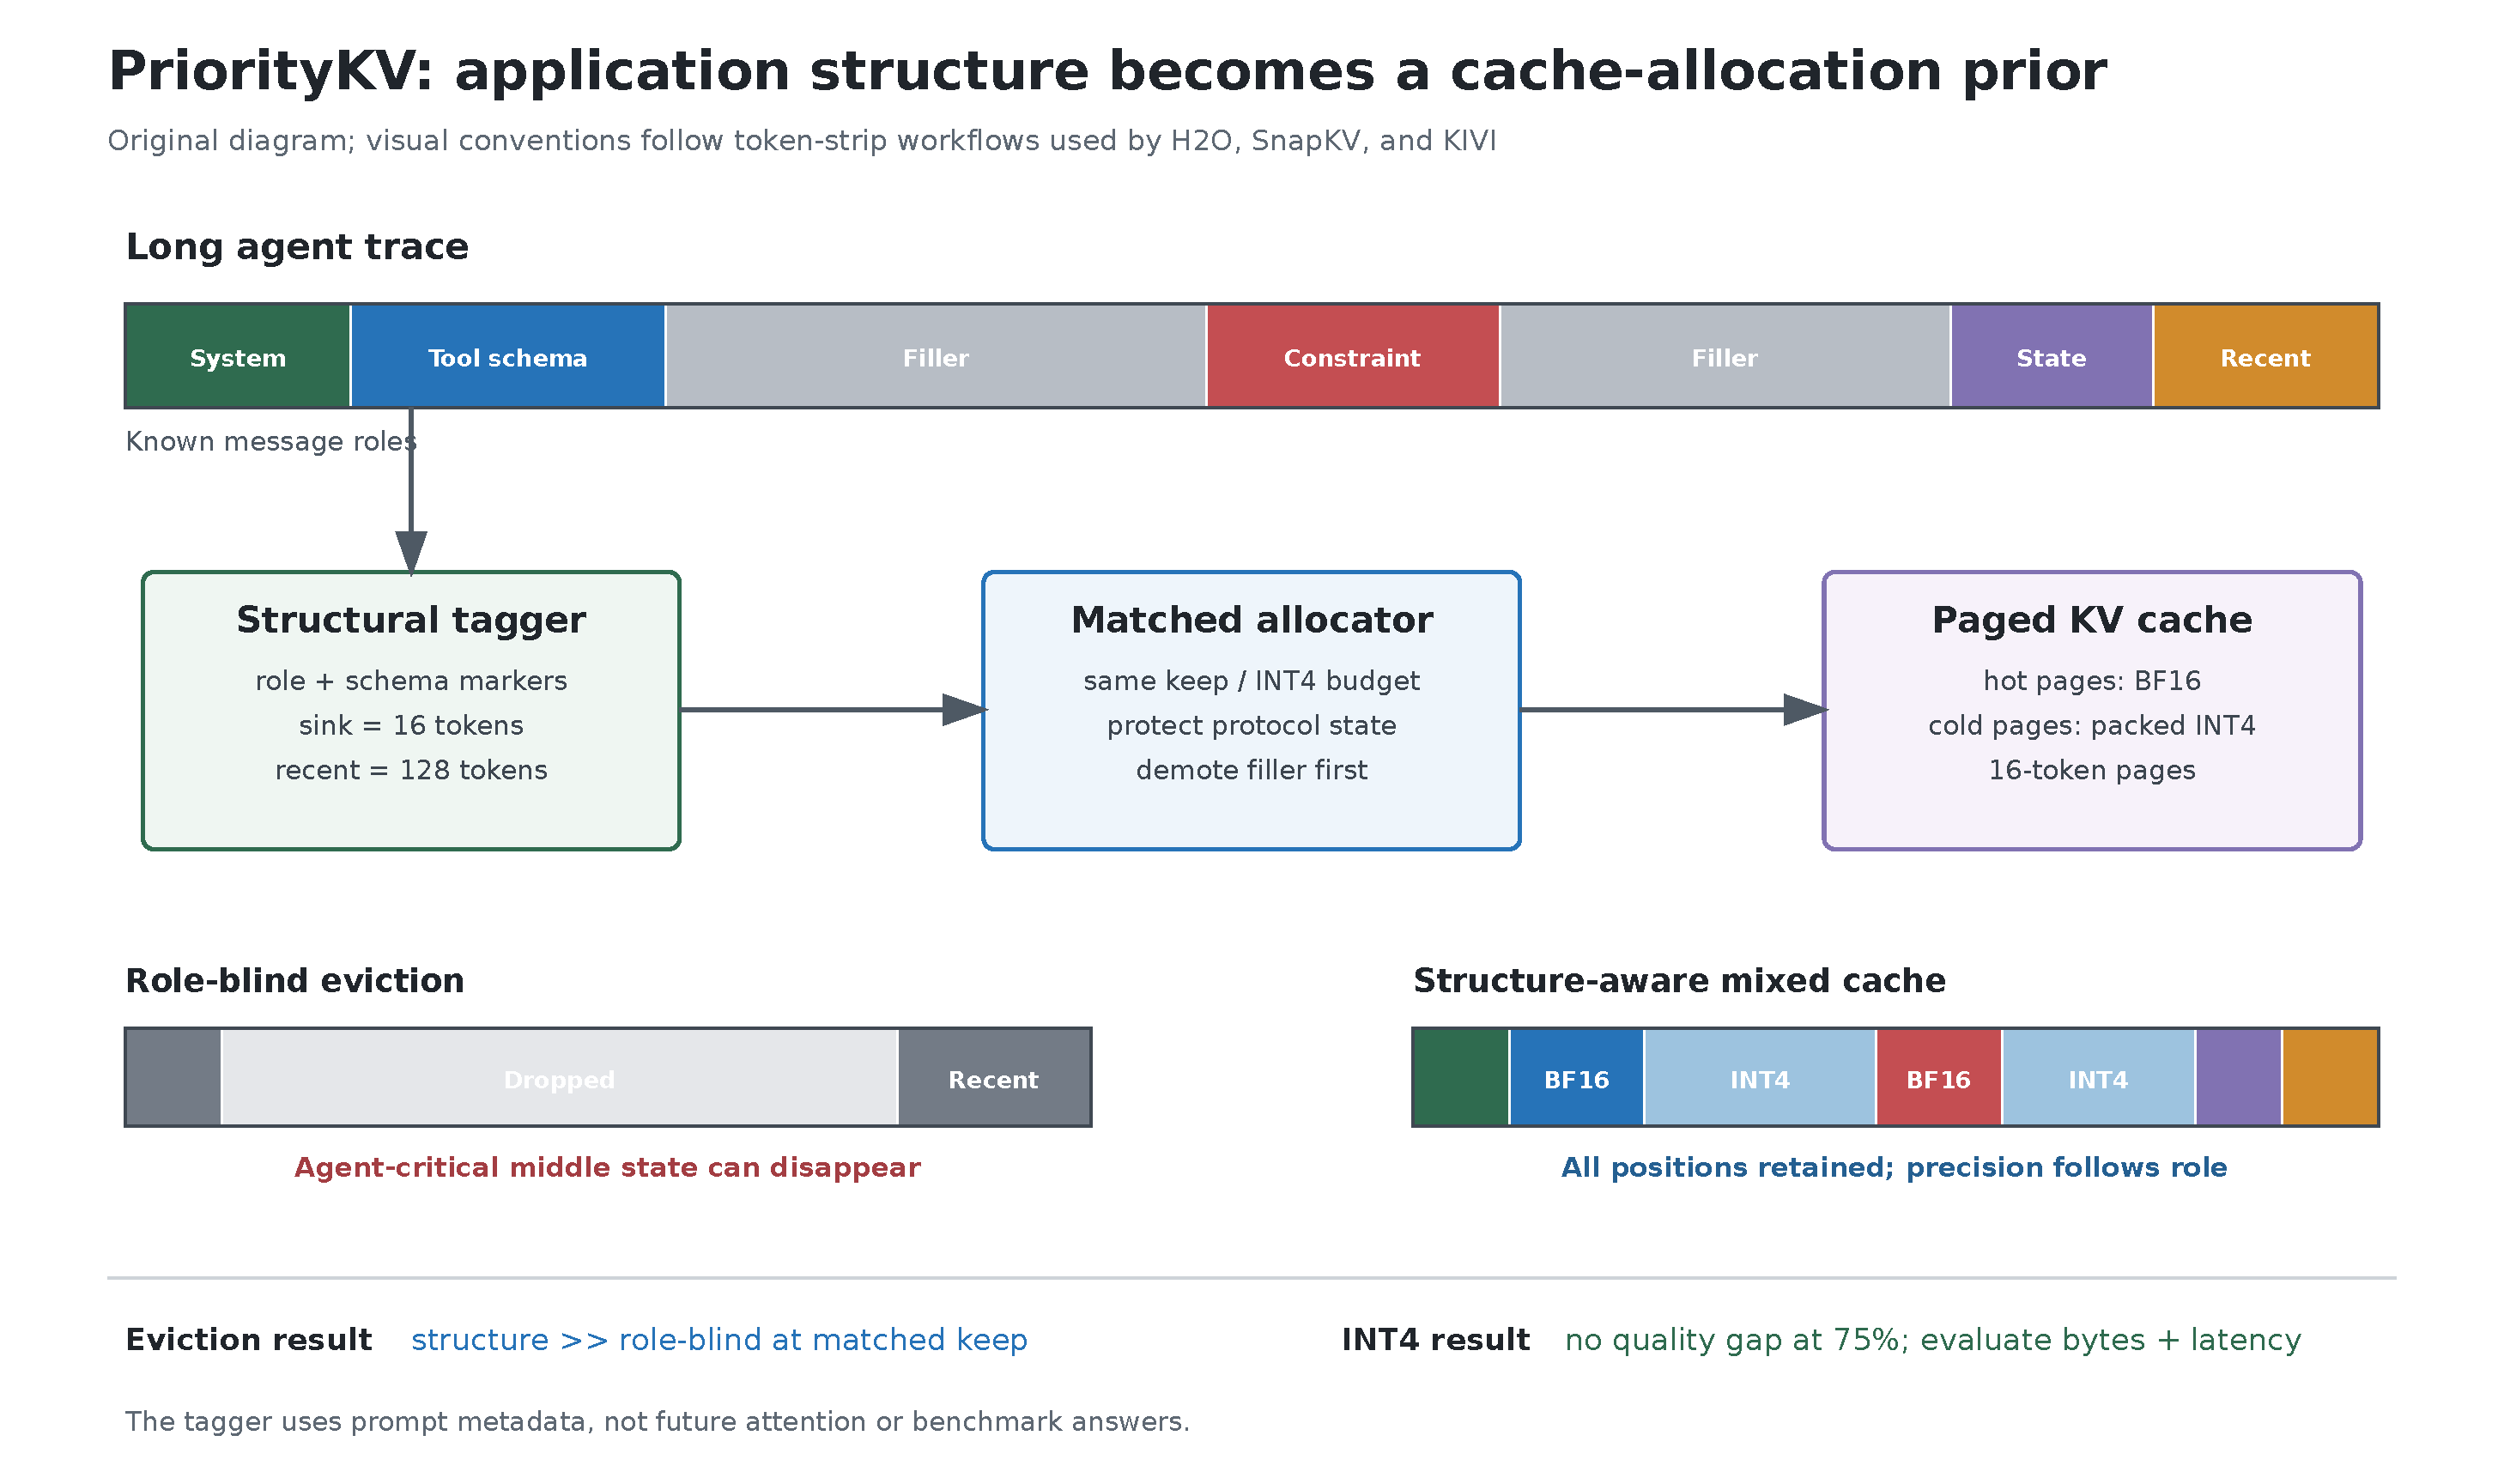
\includegraphics[keepaspectratio,alt={PriorityKV overview}]{figures/prioritykv_overview.pdf}}

Figure 1 uses the token-strip and left-to-right cache-workflow
conventions common in H2O {[}5{]}, SnapKV {[}6{]}, and KIVI {[}8{]}, but
depicts PriorityKV\textquotesingle s distinct input signal and
allocation policy. Unlike attention-derived selection, PriorityKV begins
with message-role metadata already present in an agent trace.

\section{2. Related Work}\label{2-related-work}

\textbf{KV memory management.} PagedAttention reduces fragmentation and
enables flexible KV sharing without changing which tokens are retained
{[}2{]}. StreamingLLM observes the role of attention sinks and combines
initial tokens with a recent window {[}3{]}. We use this sink-and-recent
shape as a deliberately role-blind eviction control, not as a complete
reimplementation or evaluation of StreamingLLM.

\textbf{KV eviction and token selection.} Scissorhands retains tokens
that were previously important {[}4{]}, while H2O balances heavy hitters
with recent tokens {[}5{]}. SnapKV estimates prompt importance from an
observation window {[}6{]}, and PyramidKV varies the budget across
layers {[}7{]}. These methods derive importance from model behavior.
PriorityKV instead asks whether application-visible message roles are
useful when the workload is an agent trace. The approaches are
complementary: structural priors could be combined with attention-based
selection, but that combination is not evaluated here.

\textbf{KV quantization.} KIVI motivates asymmetric low-bit treatment of
keys and values and demonstrates that aggressive KV quantization can
preserve downstream quality {[}8{]}. Our INT4 path is not proposed as a
replacement for KIVI or a new quantizer. It is a storage and measurement
vehicle for comparing role-aware and role-blind precision allocation.

\textbf{Serving and evaluation.} FlashInfer provides composable
attention kernels and state merging for heterogeneous serving workloads
{[}9{]}. PriorityKV uses \texttt{merge\_state} to combine hot BF16 and
dequantized cold attention results. LongBench and RULER provide broad
long-context evaluations {[}10, 11{]}. PriorityBench is narrower: it
isolates deterministic agent-state failures and should be read as a
complementary diagnostic rather than a general long-context benchmark.

\section{3. PriorityBench-A}\label{3-prioritybench-a}

\subsection{3.1 Tasks}\label{31-tasks}

PriorityBench-A contains 240 generated multi-turn conversations, with 80
examples in each of three categories:

{\def\LTcaptype{none} % do not increment counter
\begin{longtable}[]{@{}lll@{}}
\toprule\noalign{}
Category & Required behavior & Scoring \\
\midrule\noalign{}
\endhead
\bottomrule\noalign{}
\endlastfoot
Tool schema & Emit a valid call under an earlier tool contract & JSON
parsing plus schema-subset checks \\
Instruction supersession & Follow the latest of conflicting constraints
& Required and forbidden regular expressions \\
Multi-turn state & Reuse an earlier ID, path, or preference & Exact slot
match \\
\end{longtable}
}

Each conversation plants relevant state, adds benign filler, and ends
with a request whose correct answer depends on that state. Scoring is
programmatic and does not use an LLM-as-judge. The lock contains 83
examples at 8k, 81 at 16k, and 76 at 32k; the split counts are 92
calibration, 49 validation, and 99 test. Stable hashing assigns splits.
The manifest SHA256 is
\texttt{fc44b966725738c94008ba61ce57ad7366169b9c0be73074f8161d909ccfae89}.

PriorityBench is synthetic by design. It offers controlled failure
attribution and exact scoring, but it does not estimate the frequency of
these failures in production traffic. The generator, templates,
manifest, and scorers are included in the repository.

\subsection{3.2 Adversarial variants}\label{32-adversarial-variants}

The initial templates often place short, gold-bearing turns before long
filler. A policy that simply prefers short or early spans can therefore
appear semantic. We use two checks:

\begin{itemize}
\tightlist
\item
  \textbf{Buried state:} lengthen or bury gold-bearing turns so that
  short-turn tagging no longer identifies all state.
\item
  \textbf{Middle relocation:} move the state block away from the prefix
  while preserving the leading system message and final request.
\end{itemize}

These variants exposed a real limitation: the basic structure policy
preserves tool and constraint roles more reliably than unmarked
free-form state. We retain that failure in the results.

\section{4. Method}\label{4-method}

\subsection{4.1 Structural roles}\label{41-structural-roles}

PriorityKV maps chat messages to page roles using information already
available to an agent serving stack. System messages are tagged as
system, tool, or constraint spans; tool messages and schema-like
assistant messages are tagged as tool spans; constraint-like user
messages are tagged as constraints; and short state-bearing turns can be
tagged as other structured state. The first 16 tokens are protected as
an attention sink and the most recent 128 tokens are protected as a
decode-local window.

The current tagger is a transparent heuristic over message roles,
length, and a small set of schema or constraint markers. It is not a
learned importance model and does not inspect the benchmark answer. A
removed early implementation keyed on final-answer markup; the
buried-state and middle-relocation controls were added specifically to
detect such leakage.

\subsection{4.2 Matched-budget
eviction}\label{42-matched-budget-eviction}

For a prompt of length \texttt{n} and keep fraction \texttt{k}, every
arm receives the same nominal budget \texttt{round(k\ n)}, subject to
the common sink and recent minimum. The controls are:

\begin{itemize}
\tightlist
\item
  \textbf{Role-blind sink+recent:} retain the sink and then fill the
  budget from the recent edge.
\item
  \textbf{Random:} retain the same mandatory region and sample the
  remaining pages.
\item
  \textbf{Fixed prefix:} retain sink, recent, and the lowest-index
  pages.
\item
  \textbf{Structure-aware:} retain sink, recent, and protected-role
  pages before filling the remaining budget near the recent edge.
\item
  \textbf{Keep all:} retain the complete prompt as a wiring control.
\end{itemize}

Page experiments operate on contiguous 16-token pages. Token selection
is applied by gathering the retained prompt positions and regenerating
the cache, avoiding an invalid RoPE index substitution. These
experiments isolate missing-state sensitivity; they are not the packed
mixed-precision serving path.

\subsection{4.3 Matched mixed
precision}\label{43-matched-mixed-precision}

The mixed policy assigns the same number of positions to INT4 in both
arms. With \texttt{int4\_frac\ =\ 0.75}, sink and recent positions
remain BF16. The role-blind arm spaces INT4 positions uniformly through
the demotable region. The structure arm demotes filler and low-risk
roles first, spilling into protected roles only when required to meet
the exact budget.

For the frozen Qwen3-8B path, K and V are divided into 16-token pages.
Hot pages store BF16 tensors; cold pages store packed 4-bit values and
per-group scale metadata. Packing is real storage, not a fake-quantized
BF16 tensor. The implementation reports both actual payload bytes,
including metadata, and an idealized 0.5-byte-per-element model.

\subsection{4.4 FlashInfer decode}\label{44-flashinfer-decode}

Prefill uses the native Hugging Face path. The cache is then split into
hot BF16 pages and cold packed pages. During decode, the Qwen3 attention
shim performs at most two attention calls per layer: one over coalesced
hot pages and the decode tail, and one over cold pages after
dequantization. FlashInfer\textquotesingle s log-sum-exp merge combines
their attention states. Parity tests reduced the maximum absolute merge
error to approximately \texttt{4.88e-4} after correcting an LSE-base
mismatch.

The current implementation expands cold INT4 pages into a BF16 GPU
scratch buffer before attention. This avoids silently materializing a
full Hugging Face cache but limits peak memory savings and adds decode
overhead. Direct fused or page-streamed INT4 attention is future systems
work.

\pandocbounded{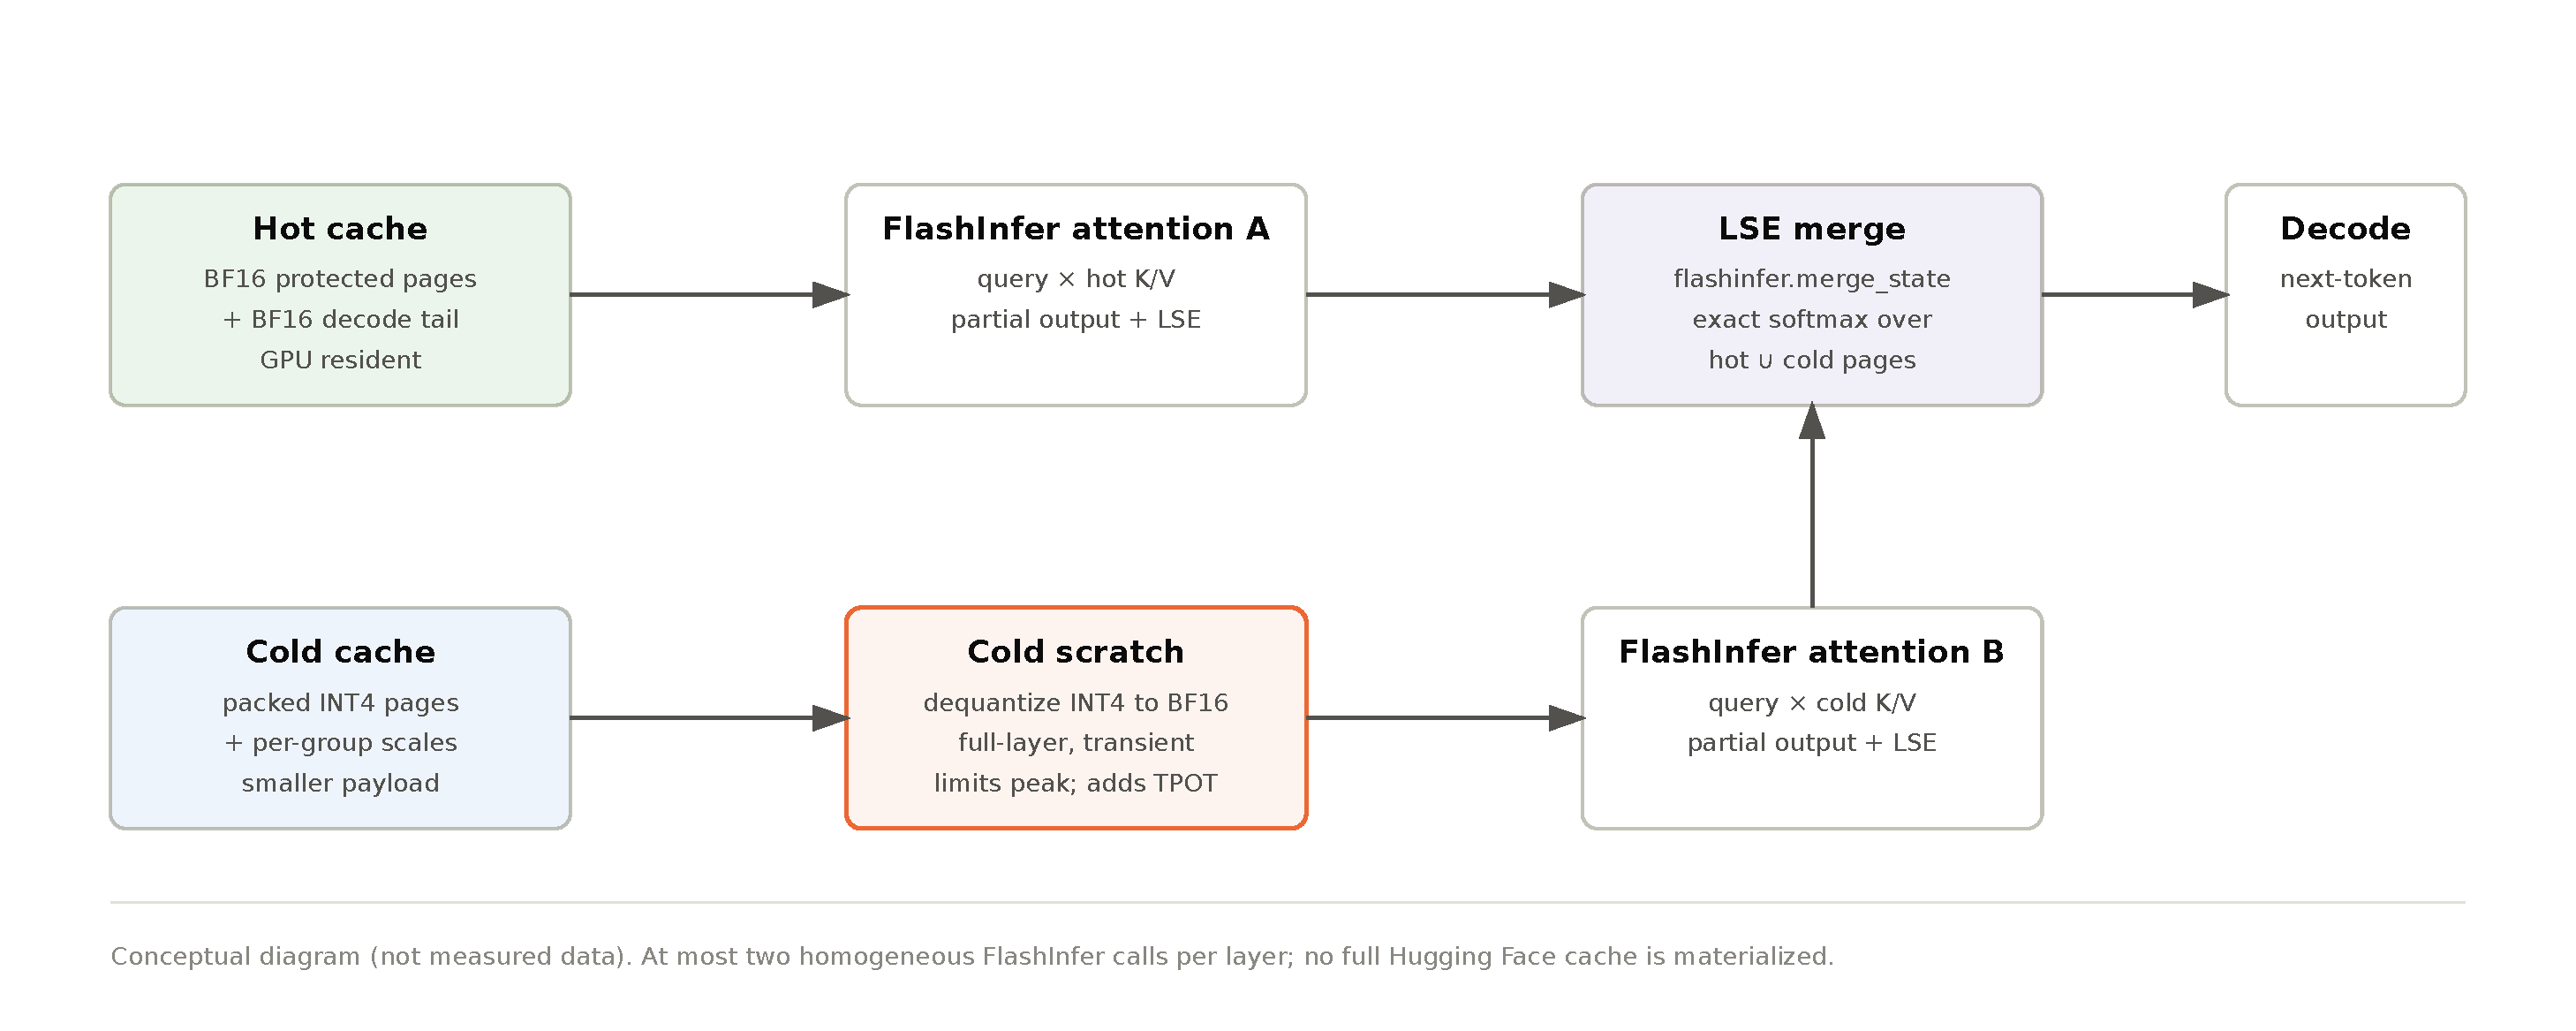
\includegraphics[keepaspectratio,alt={FlashInfer decode dataflow}]{figures/flashinfer_decode_dataflow.pdf}}

Figure 2 follows the modular system-dataflow convention used by
FlashInfer {[}9{]} and the grouped/residual cache presentation used by
KIVI {[}8{]}. It makes the temporary BF16 cold scratch explicit because
that allocation explains the difference between payload and peak memory.

\section{5. Experimental Setup}\label{5-experimental-setup}

The primary experiments use Qwen3-8B in non-thinking greedy decode mode
on NVIDIA H200 GPUs. The model revision, benchmark hash, configurations,
job IDs, and job status are frozen in
\texttt{FINAL\_RUN\_MANIFEST.yaml}.

The evaluation families answer different questions:

{\def\LTcaptype{none} % do not increment counter
\begin{longtable}[]{@{}lrl@{}}
\toprule\noalign{}
Family & Size & Purpose \\
\midrule\noalign{}
\endhead
\bottomrule\noalign{}
\endlastfoot
Matched-keep stress & 14--16 examples per configuration & Controlled
eviction sensitivity and policy ablations \\
Lock-240 mixed quality & 240 examples & Quality of FullKV and matched
75\% INT4 placement \\
D4 latency & 18 examples, 9 per 8k/16k stratum & Pack, cold-scratch,
TTFT, and TPOT measurement \\
Peak and payload & 18 examples & Allocated/reserved CUDA peak and cache
payload \\
Gemma reduced & 14 examples at approximately 8k & Directional
second-model check only \\
\end{longtable}
}

Latency rows use 128 generated tokens, greedy decoding, one warm-up
sequence, and three timing repeats whose median is recorded. FullKV uses
SDPA; mixed arms use the FlashInfer shim. This is a single-request
prototype comparison, not a throughput or concurrency study. The FP8
publish job uses a different batch-amortized timing protocol and is
therefore retained as a pass/fail secondary check rather than merged
into the main latency table.

\section{6. Results}\label{6-results}

\subsection{6.1 Structure matters under
eviction}\label{61-structure-matters-under-eviction}

{\def\LTcaptype{none} % do not increment counter
\begin{longtable}[]{@{}lrrrrr@{}}
\toprule\noalign{}
Setting & n & Full/keep-all & Role-blind & Random/fixed prefix &
Structure \\
\midrule\noalign{}
\endhead
\bottomrule\noalign{}
\endlastfoot
Token keep, \texttt{k=0.25} & 14 & 1.000 & 0.000 & random 0.000 &
\textbf{1.000} \\
Page keep, \texttt{k=0.15} & 14 & 1.000 & 0.000 & random 0.071 &
\textbf{0.643} \\
Page keep, \texttt{k=0.25} & 14 & 1.000 & 0.000 & random 0.286 &
\textbf{0.643} \\
Page keep, \texttt{k=0.35} & 14 & 1.000 & 0.000 & random 0.429 &
\textbf{0.643} \\
Buried token state, \texttt{k=0.25} & 14 & 1.000 & 0.000 & random 0.000
& \textbf{0.429} \\
Middle-relocated page state, \texttt{k=0.25} & 16 & 1.000 & 0.000 &
fixed prefix 0.125 & \textbf{0.688} \\
\end{longtable}
}

The same 14-example slice is reused across the page-budget sweep, so the
rows are an ablation rather than independent replications. The uniform
arm\textquotesingle s zero score shows that the sink-and-recent policy
removes required middle state at these aggressive budgets. The structure
arm\textquotesingle s 0.643 plateau and buried-state drop are equally
important: explicit roles rescue a subset of failures, but the heuristic
does not identify all free-form multi-turn state. Middle relocation
separates structure from the fixed-prefix control, showing that the
result is not solely early-position retention.

\pandocbounded{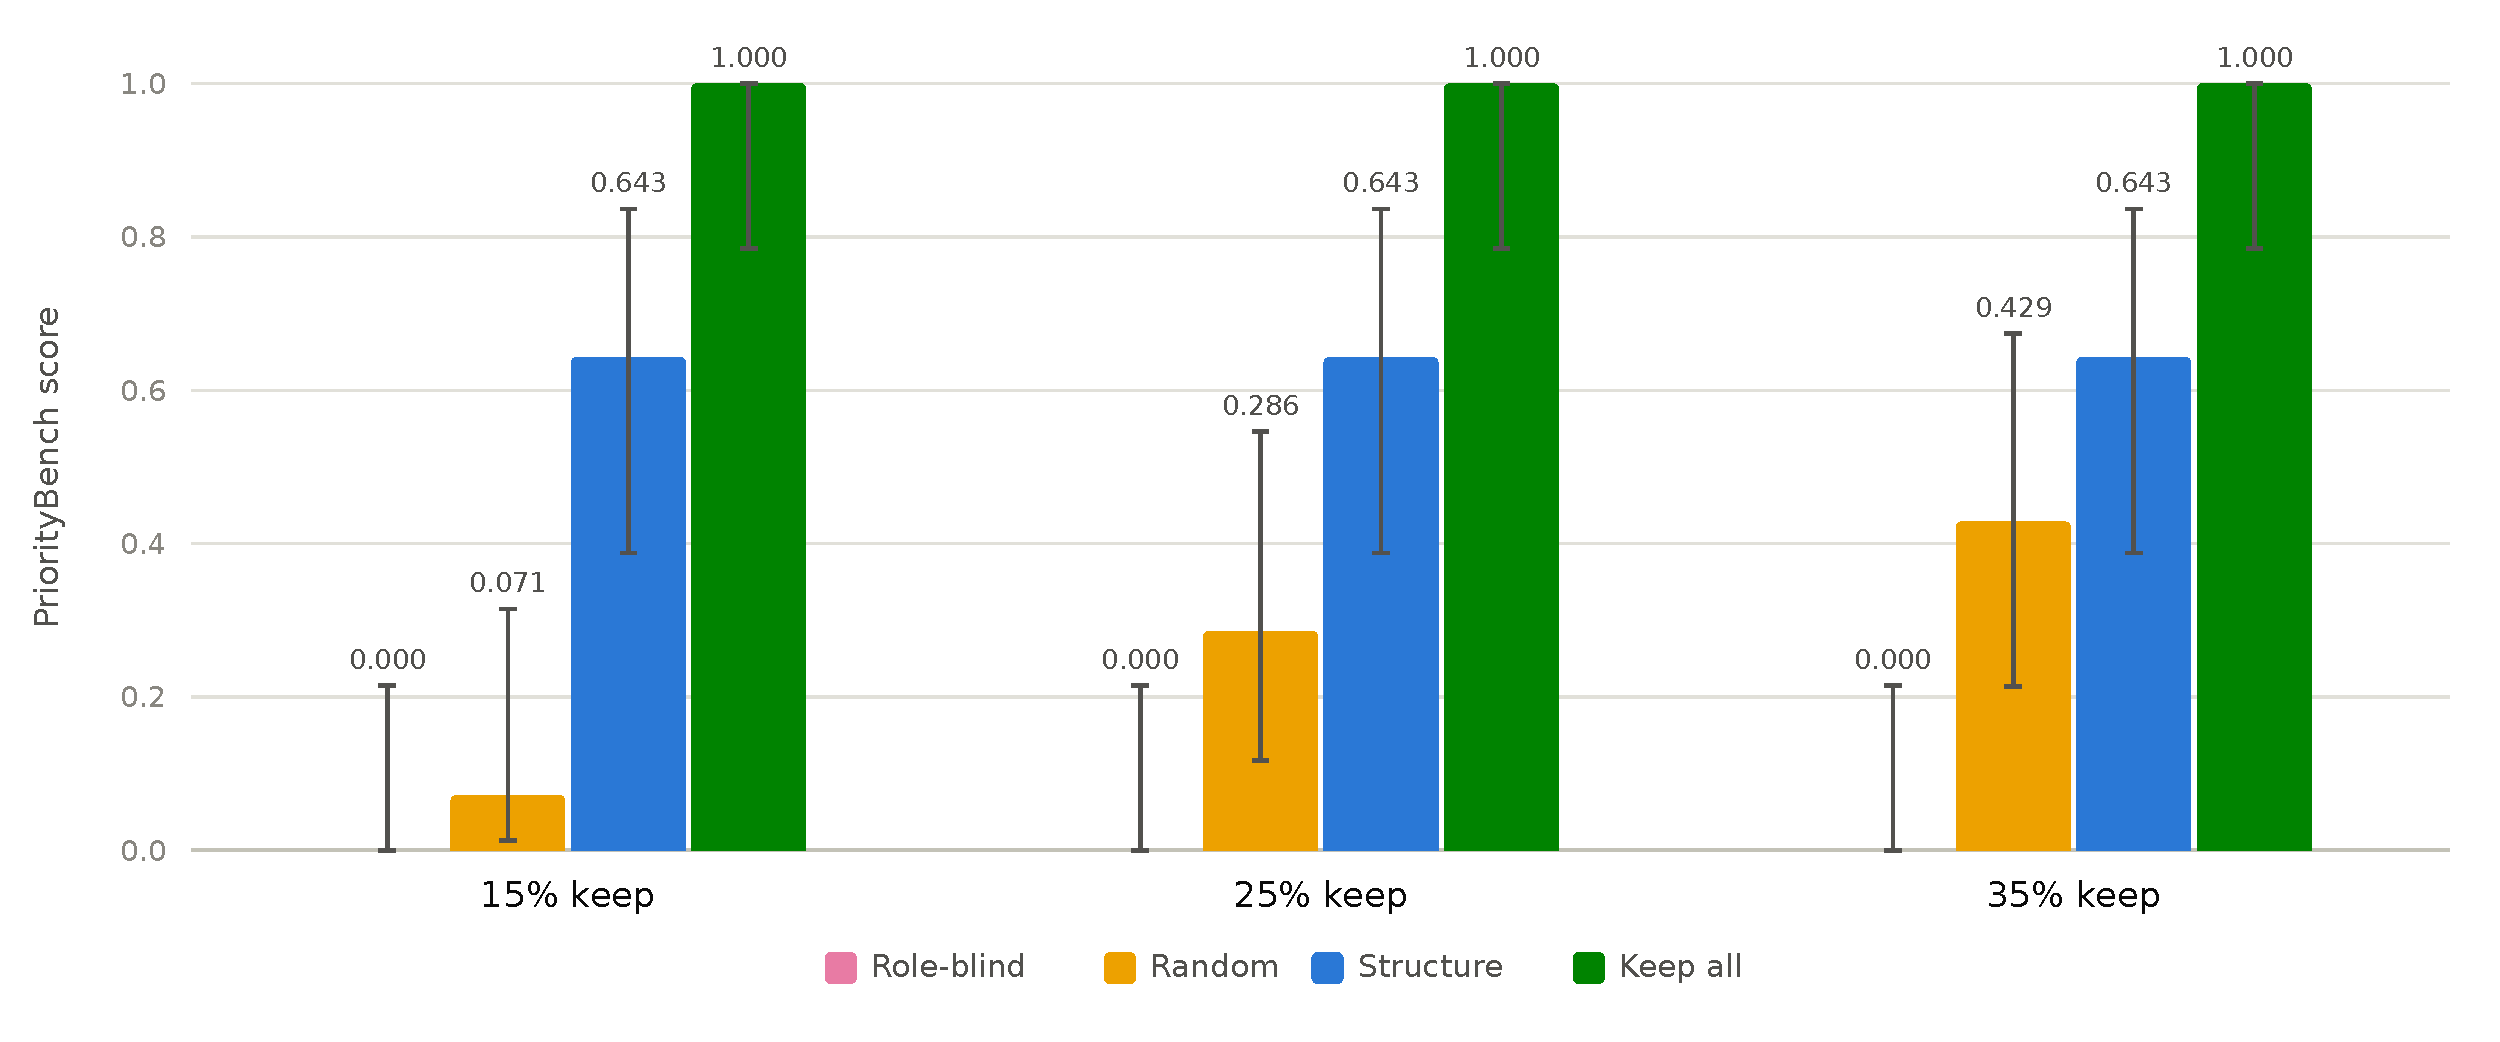
\includegraphics[keepaspectratio,alt={Matched keep-budget results}]{figures/reliability_keep_sweep.pdf}}

\subsection{6.2 Soft INT4 does not create a quality
separation}\label{62-soft-int4-does-not-create-a-quality-separation}

{\def\LTcaptype{none} % do not increment counter
\begin{longtable}[]{@{}lrr@{}}
\toprule\noalign{}
Arm & Score, n=240 & Difference from FullKV \\
\midrule\noalign{}
\endhead
\bottomrule\noalign{}
\endlastfoot
FullKV & \textbf{0.8875} & -- \\
Role-blind mixed INT4 & \textbf{0.8792} & -0.0083 \\
Structure-aware mixed INT4 & \textbf{0.8833} & -0.0042 \\
\end{longtable}
}

The structure and role-blind arms differ by 0.0042, equivalent to one
aggregate success on this 240-example benchmark. We do not interpret
that difference as evidence of a structure-aware quantization quality
advantage. At 8k and 16k, all three arms score 1.0. At 32k, FullKV
itself falls to 0.645, while role-blind and structure-aware mixed score
0.618 and 0.632. The primary conclusion is negative: retaining an INT4
approximation of 75\% of positions is much less destructive than
evicting those positions.

\pandocbounded{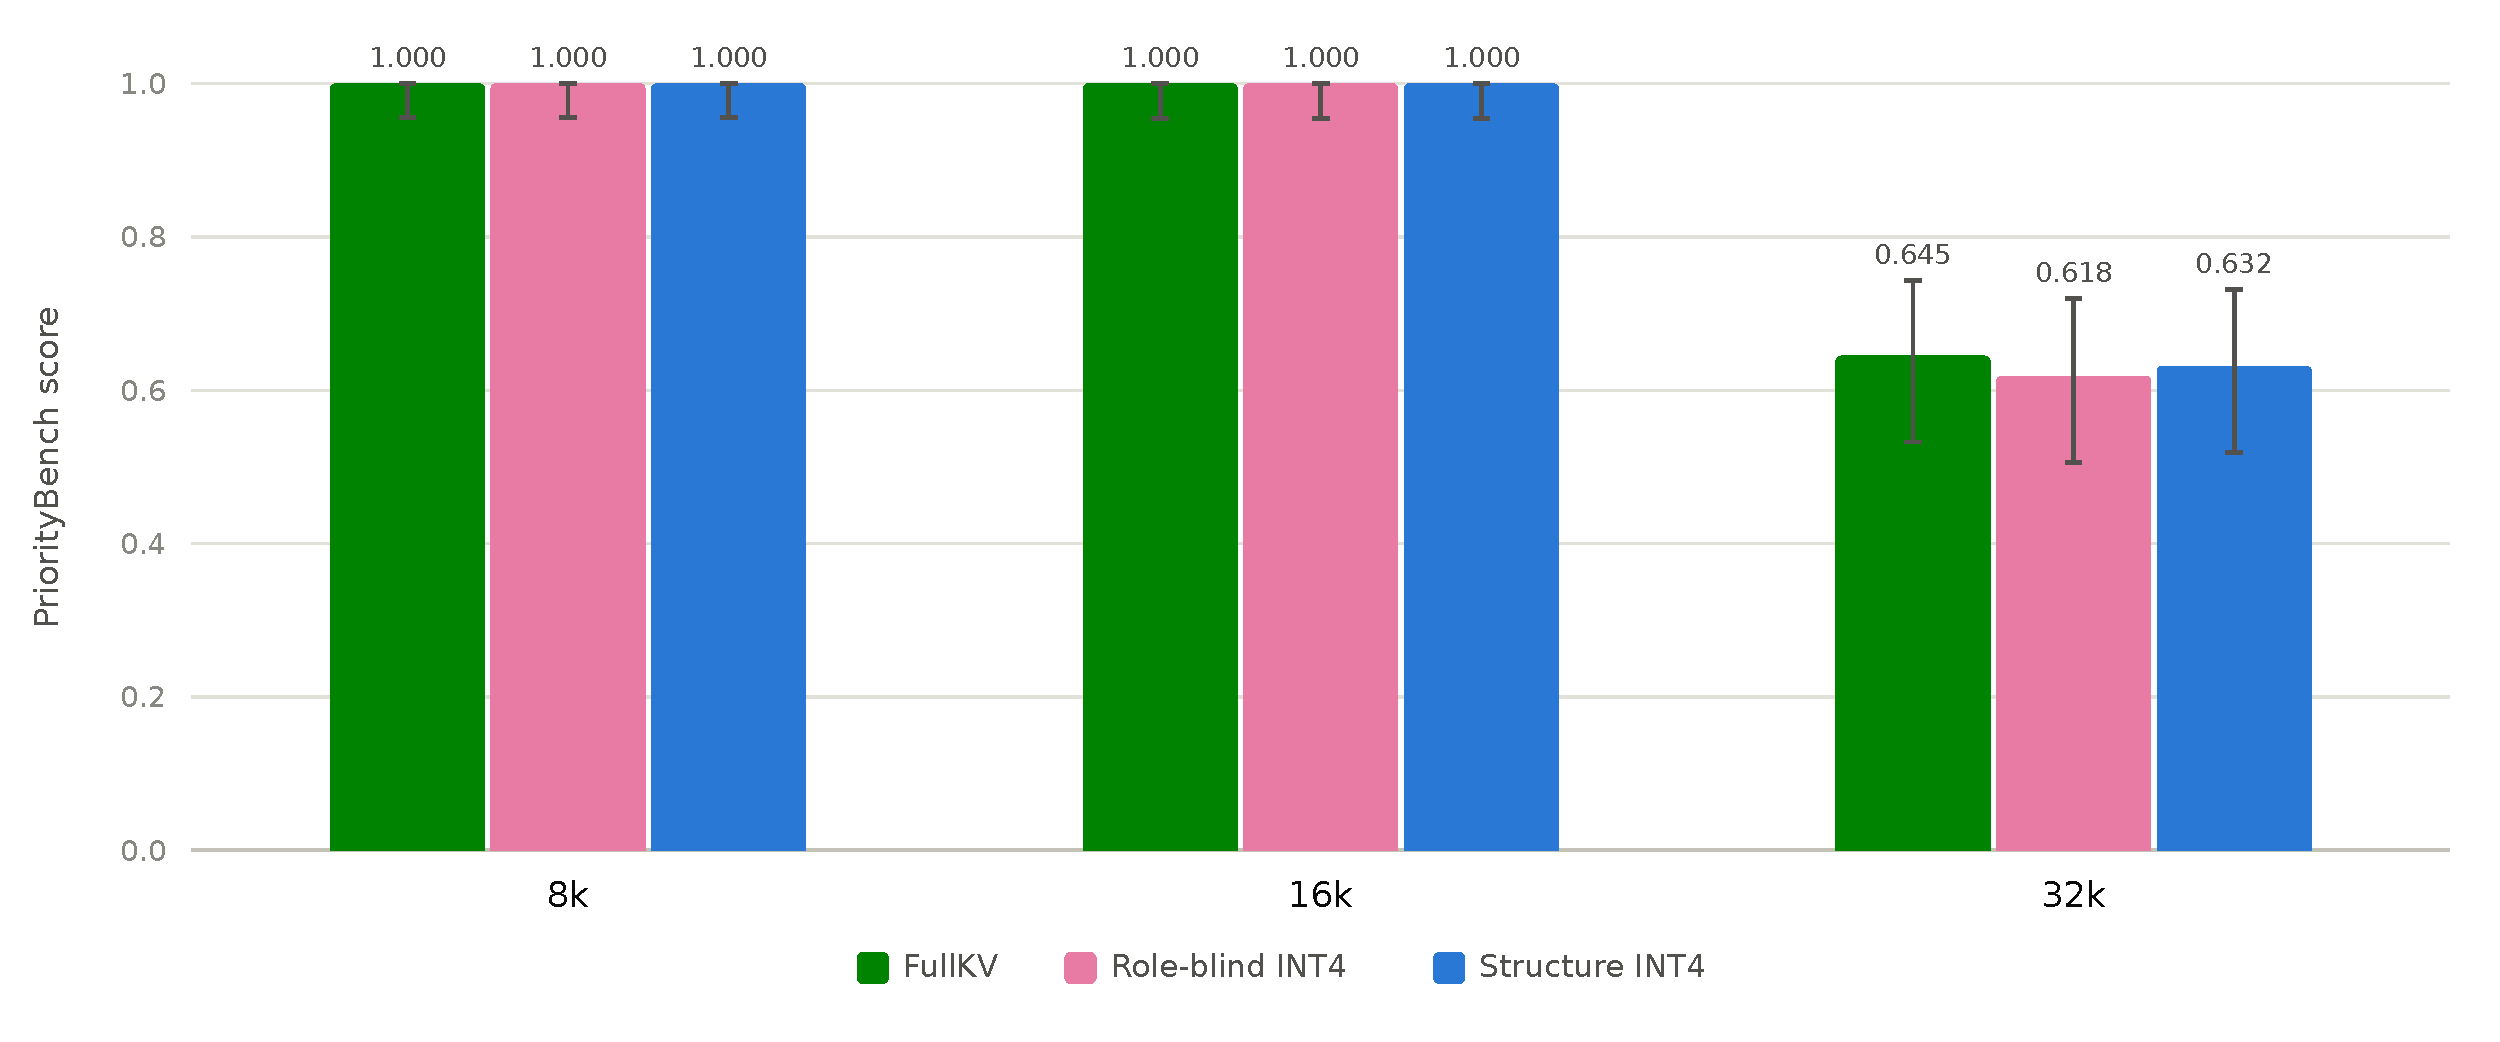
\includegraphics[keepaspectratio,alt={Lock-240 quality by context length}]{figures/lock240_quality_by_length.pdf}}

\subsection{6.3 Packed storage reduces bytes, not
latency}\label{63-packed-storage-reduces-bytes-not-latency}

{\def\LTcaptype{none} % do not increment counter
\begin{longtable}[]{@{}lrrrrr@{}}
\toprule\noalign{}
Context & Structure pack & Cold scratch & E2E / FullKV & TPOT / FullKV &
Score \\
\midrule\noalign{}
\endhead
\bottomrule\noalign{}
\endlastfoot
8k & 34.8 ms & 14.2 ms & 1.118x & 1.200x & 1.000 \\
16k & 48.1 ms & 19.7 ms & 1.113x & 1.215x & 0.889 \\
\end{longtable}
}

The mixed path is close to FullKV in end-to-end latency because prefill
dominates these single-request traces, but it is approximately 20\%
slower per output token. This is a latency cost, not a speedup. Packing
and cold-scratch construction cost tens of milliseconds per sequence.

Across the 18-example memory slice, FullKV allocates 23.61 GB at peak
and the structure-aware mixed path allocates 20.50 GB, a ratio of 0.868.
Actual mixed payload is 1.679 GB versus a 2.336 GB BF16 cache model, a
ratio of 0.719. The idealized bit model is 0.473. The smaller payload
does not translate one-for-one into peak reduction because the cold
attention path temporarily expands INT4 pages to BF16.

\pandocbounded{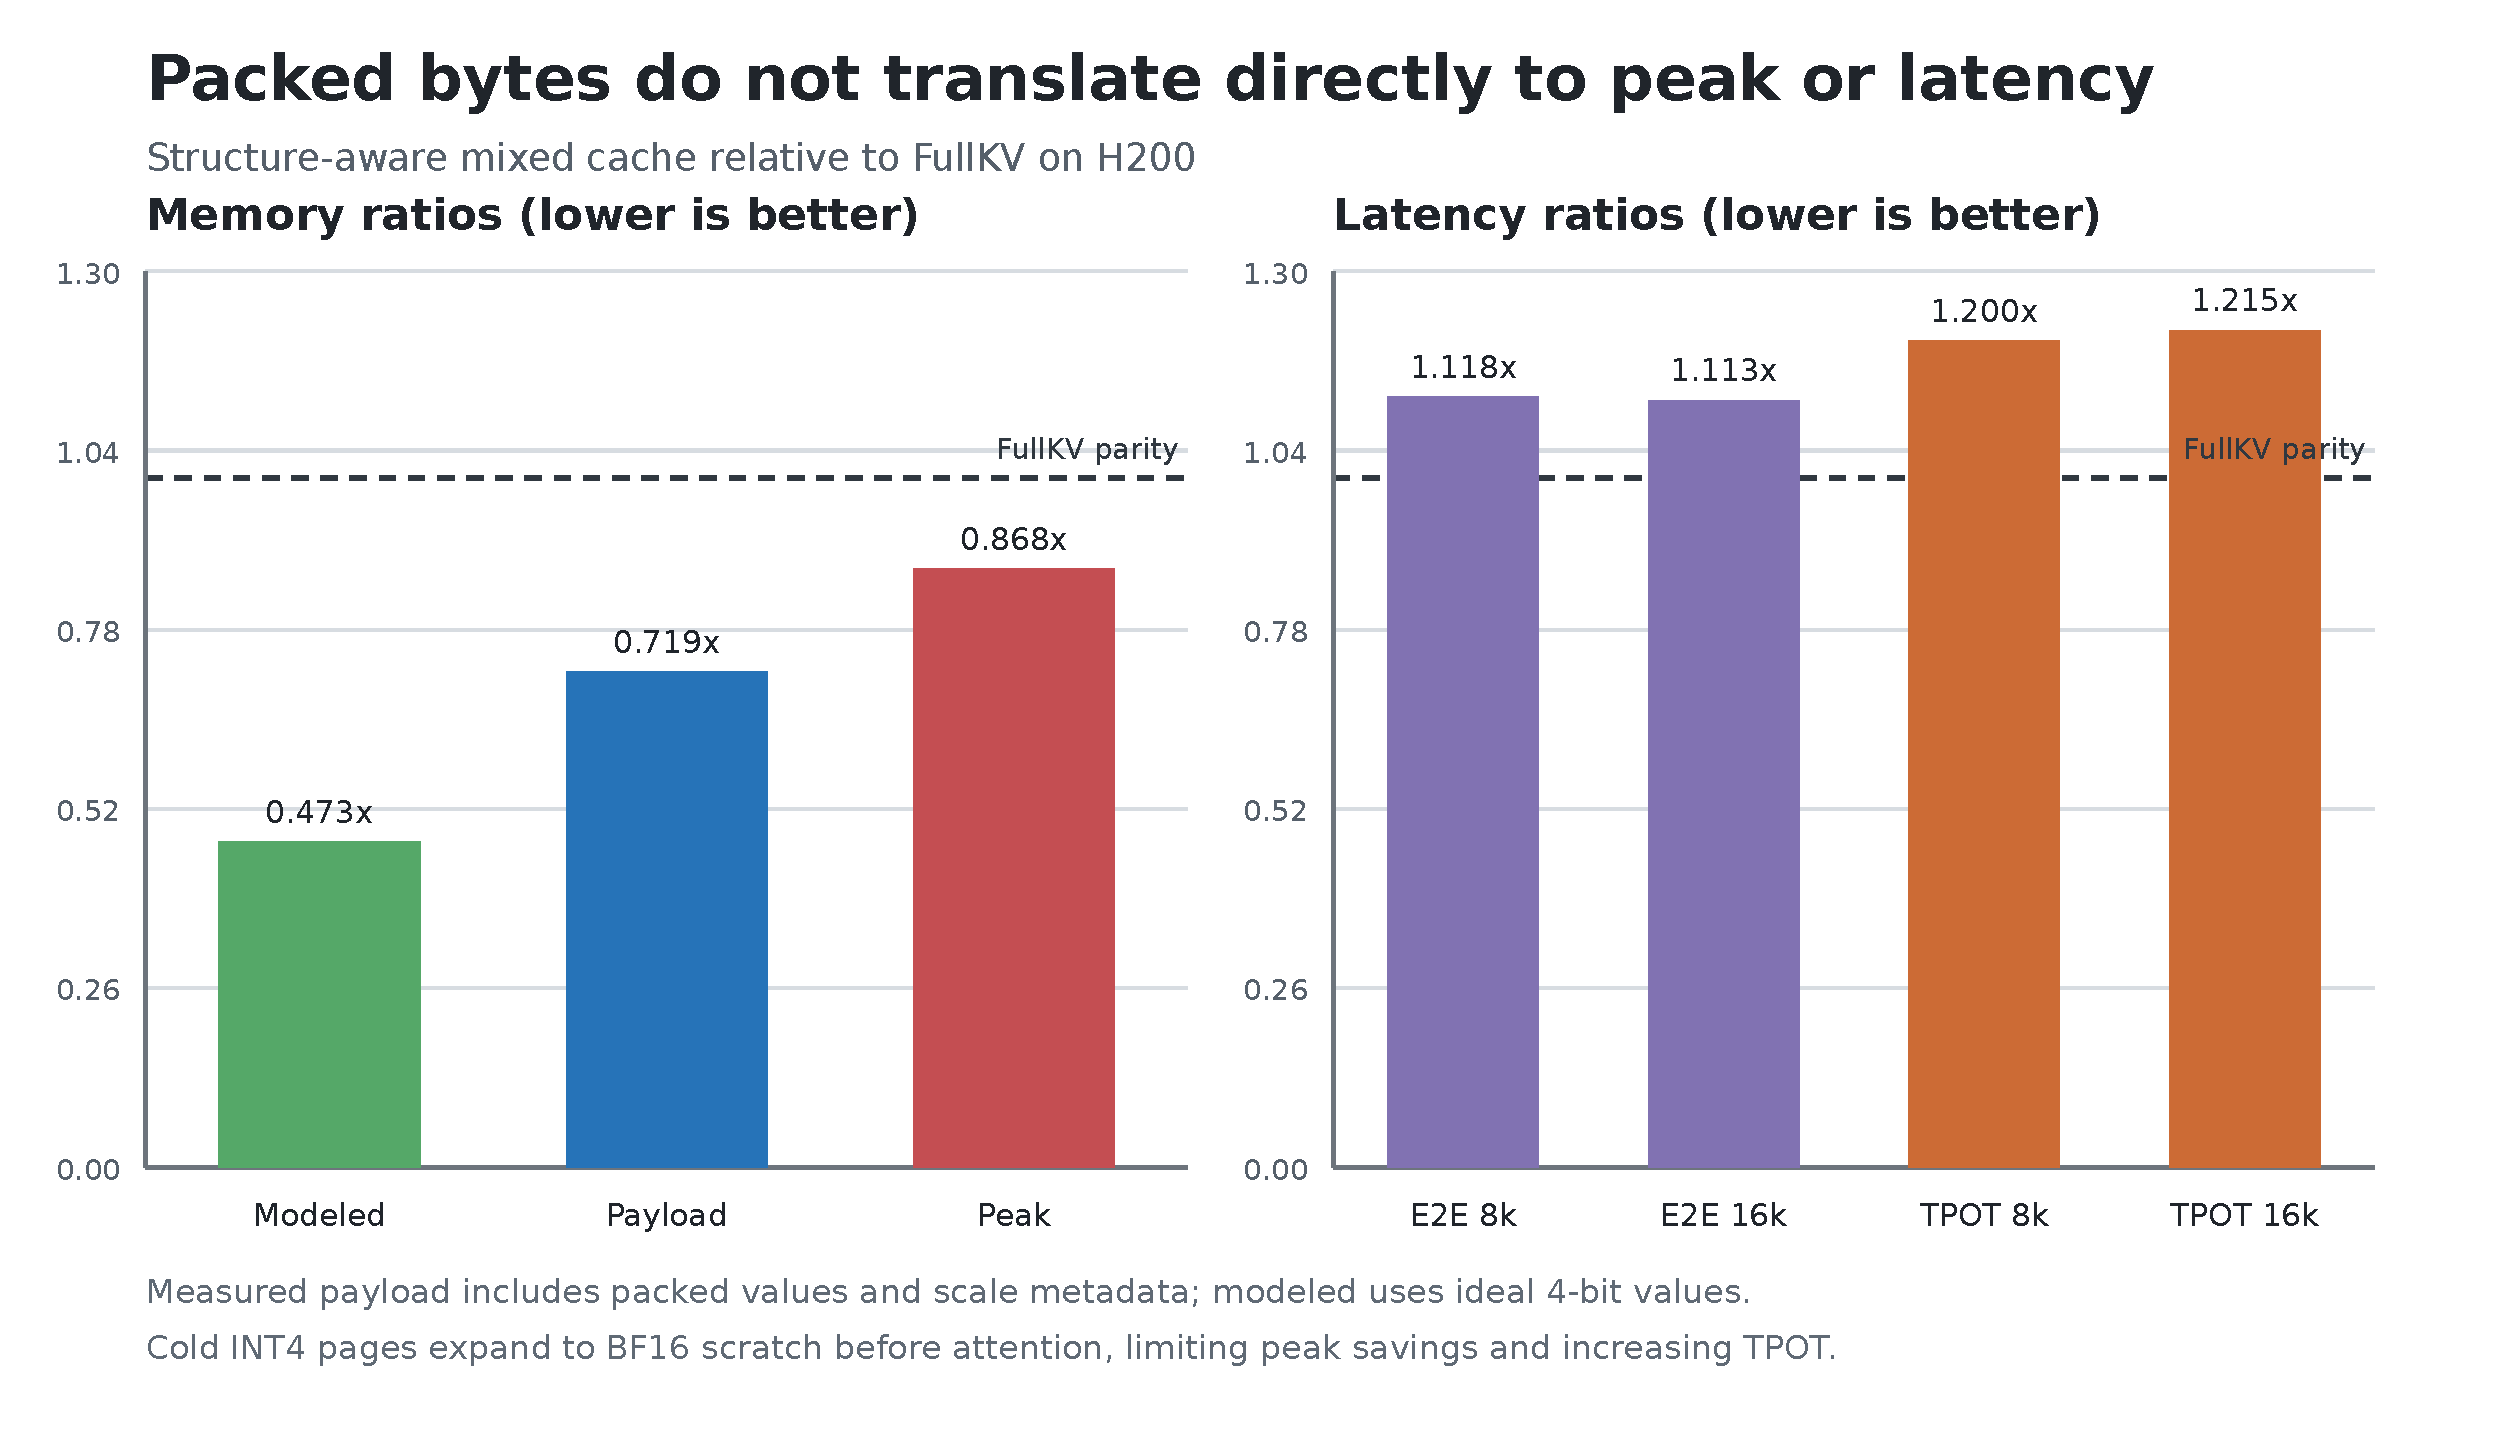
\includegraphics[keepaspectratio,alt={Systems tradeoff}]{figures/systems_tradeoff.pdf}}

\subsection{6.4 Secondary model check}\label{64-secondary-model-check}

On a reduced 14-example Gemma-2-9B-IT check at approximately 8k, FullKV,
structure, and role-blind eviction score 0.357, 0.143, and 0.000. This
supports only the direction
\texttt{structure\ \textgreater{}=\ role-blind} under the tested stress.
The absolute values are not comparable to the Qwen lock because the
prompt/scorer design and length cap were tuned around Qwen.

\section{7. Discussion}\label{7-discussion}

The experiments support a narrow design principle: when an application
already knows the protocol role of a span, discarding that information
before cache allocation is unnecessary. Message roles are cheap,
deterministic priors that can protect tool and instruction state when
attention-only importance estimates are unavailable or stale.

The results also show why eviction and quantization should not be
grouped under a single "compression quality" claim. In our setup,
removing 75\% of tokens destroys the targeted agent behaviors, while
representing approximately 75\% of positions in INT4 leaves the
aggregate result near FullKV. A mixed-precision policy should therefore
be justified by memory and kernel behavior unless a harder quality
regime demonstrates otherwise.

Finally, payload accounting is not a proxy for deployed memory or
performance. The prototype stores fewer bytes but re-expands cold pages
for attention. A production implementation would need fused low-bit
attention or bounded page streaming, allocator analysis under
concurrency, and integration into a serving scheduler before claiming
capacity or throughput gains.

\section{8. Limitations and Threats to
Validity}\label{8-limitations-and-threats-to-validity}

\begin{enumerate}
\def\labelenumi{\arabic{enumi}.}
\tightlist
\item
  \textbf{Synthetic benchmark.} PriorityBench provides controlled,
  deterministic failures but is not sampled from production agent
  traffic.
\item
  \textbf{Small positive-result slices.} The decisive eviction
  experiments use 14--16 examples. The 240-example run evaluates mixed
  INT4 quality, not matched eviction.
\item
  \textbf{One primary model and device.} Qwen3-8B on H200 is the only
  complete matrix. The Gemma check is reduced and low-scoring.
\item
  \textbf{Heuristic structure labels.} Free-form state without
  recognizable roles remains a failure mode. Structural metadata can
  also be missing or incorrect in real systems.
\item
  \textbf{Limited baselines.} Role-blind sink/recent, random,
  fixed-prefix, FP8, and a reduced SnapKV attempt do not constitute a
  full comparison with H2O, SnapKV, PyramidKV, or state-of-the-art KV
  quantizers.
\item
  \textbf{Prototype timing.} Measurements cover single-request latency,
  not batching, concurrency, throughput, or tail latency. FullKV SDPA
  and mixed FlashInfer are not a kernel-isolated comparison.
\item
  \textbf{Cold scratch.} INT4-to-BF16 expansion limits the realized
  peak-memory reduction and causes the measured TPOT regression.
\item
  \textbf{No uncertainty from repeated jobs.} Per-example timing medians
  reduce local noise, but canonical jobs were not repeated across
  independent machine runs.
\end{enumerate}

PriorityBench contains generated tool contracts and synthetic
identifiers rather than personal data. The main foreseeable misuse is
overgeneralizing the benchmark to claim production reliability; the
frozen claim and public limitations are intended to prevent that
interpretation.

\section{9. Reproducibility}\label{9-reproducibility}

The repository records:

\begin{itemize}
\tightlist
\item
  benchmark generator, templates, scorers, manifest, and SHA256 audit;
\item
  exact Qwen3-8B model revision and non-thinking generation settings;
\item
  frozen YAML configurations and job commands;
\item
  raw summaries, logs, and GPU snapshots for the main latency, memory,
  quality, and Gemma jobs;
\item
  CPU unit tests for policies, packed storage, quantization, page
  management, and FlashInfer state logic; and
\item
  \texttt{FINAL\_RUN\_MANIFEST.yaml} as the claim and artifact index.
\end{itemize}

Generate and audit the locked dataset with:

\begin{Shaded}
\begin{Highlighting}[]
\VariableTok{PYTHONPATH}\OperatorTok{=}\NormalTok{src }\ExtensionTok{uv}\NormalTok{ run python scripts/mk\_bench.py }\AttributeTok{{-}{-}mode}\NormalTok{ w3\_lock}
\VariableTok{PYTHONPATH}\OperatorTok{=}\NormalTok{src }\ExtensionTok{uv}\NormalTok{ run python scripts/audit\_bench.py}
\end{Highlighting}
\end{Shaded}

Regenerate the paper figures from frozen artifacts with:

\begin{Shaded}
\begin{Highlighting}[]
\ExtensionTok{uv}\NormalTok{ run python scripts/make\_publication\_figures.py}
\end{Highlighting}
\end{Shaded}

GPU reproduction requires the pinned model weights, the \texttt{gpu}
optional dependency set, and an H200-class CUDA environment. Canonical
commands and result bundles are documented under \texttt{jobs/} and in
\texttt{docs/REPRODUCIBILITY.md}.

\section{10. Conclusion}\label{10-conclusion}

PriorityKV demonstrates that known agent-trace structure is a useful
cache-allocation signal under aggressive eviction. It does not
demonstrate that role-aware soft INT4 placement improves quality, and it
does not hide that the current packed implementation is slower per
decoded token. The complete result is therefore a measurement result
rather than a universal cache-compression claim: preserve
protocol-critical state when dropping KV, use low precision for bytes
when quality permits, and measure payload, peak, and latency as separate
quantities.

\section{References}\label{references}

\begin{enumerate}
\def\labelenumi{\arabic{enumi}.}
\tightlist
\item
  Vaswani et al. \emph{Attention Is All You Need.} NeurIPS, 2017.
\item
  Kwon et al. \emph{Efficient Memory Management for Large Language Model
  Serving with PagedAttention.} SOSP, 2023.
  \url{https://arxiv.org/abs/2309.06180}
\item
  Xiao et al. \emph{Efficient Streaming Language Models with Attention
  Sinks.} ICLR, 2024. \url{https://arxiv.org/abs/2309.17453}
\item
  Liu et al. \emph{Scissorhands: Exploiting the Persistence of
  Importance Hypothesis for LLM KV Cache Compression at Test Time.}
  NeurIPS, 2023. \url{https://arxiv.org/abs/2305.17118}
\item
  Zhang et al. \emph{H2O: Heavy-Hitter Oracle for Efficient Generative
  Inference of Large Language Models.} NeurIPS, 2023.
  \url{https://arxiv.org/abs/2306.14048}
\item
  Li et al. \emph{SnapKV: LLM Knows What You Are Looking for Before
  Generation.} NeurIPS, 2024. \url{https://arxiv.org/abs/2404.14469}
\item
  Cai et al. \emph{PyramidKV: Dynamic KV Cache Compression Based on
  Pyramidal Information Funneling.}
  \url{https://arxiv.org/abs/2406.02069}
\item
  Liu et al. \emph{KIVI: A Tuning-Free Asymmetric 2bit Quantization for
  KV Cache.} ICML, 2024. \url{https://arxiv.org/abs/2402.02750}
\item
  Ye et al. \emph{FlashInfer: Efficient and Customizable Attention
  Engine for LLM Inference Serving.}
  \url{https://arxiv.org/abs/2501.01005}
\item
  Bai et al. \emph{LongBench: A Bilingual, Multitask Benchmark for Long
  Context Understanding.} ACL, 2024.
  \url{https://arxiv.org/abs/2308.14508}
\item
  Hsieh et al. \emph{RULER: What\textquotesingle s the Real Context Size
  of Your Long-Context Language Models?} COLM, 2024.
  \url{https://arxiv.org/abs/2404.06654}
\item
  Yang et al. \emph{Qwen3 Technical Report.}
  \url{https://arxiv.org/abs/2505.09388}
\end{enumerate}

\end{document}
